% questions.tex —— 1977 年·江苏无锡市初试卷 · 题目内容片段（无答案）
% 由 tools/generate_projects.py 依来源总账自 1977/1977_数学真题_江苏无锡市初试_试题.md 生成，勿手改（改源 MD 后重跑）


\gkpart{江苏无锡市初试卷}

\begin{gktip}
\textbf{来源说明}：本题面依据固定源 PDF《1977江苏无锡市初试》全部 3 页逐题转录。源 PDF 为 1977 年高考试题汇编的书页扫描：首页顶部印有汇编章节标题「三、无锡市」，试卷本体无标题，本库 H1 为编者拟定；书页码 233、234 可见（第 3 页未见页码），第一大题第 1 小问跨第 1—2 页。原卷大题以中文数字「一、」至「九、」编号并在题名后标注分值，大题内小题以阿拉伯数字「1.」编号；本库统一转写为大题 \texttt{\textbf{N．}}（阿拉伯数字）、小问 \texttt{（N）}。全卷 9 个大题，分值 $18+16+11+8+8+8+11+8+12=100$ 分，无附加题、无参考题。原卷第三大题第 3 小问印作「当 $x$ 为何值时」，按字面保留并加源注（见该题）。扫描件未附答案，配套答案与解析为本库编者独立推导，\textbf{非官方标准答案}。
\end{gktip}

\par\medskip

\begin{question}
\gkti{1}\textbf{（18 分）} 回答下列问题：

（1） 求代数式 $f(x)=3x^2-2x-5$ 的值，当 $x=0$ 时，$f(0)=\underline{\hspace{2.5em}}$；当 $x=-1$ 时，$f(-1)=\underline{\hspace{2.5em}}$；当 $x=\dfrac18$ 时，$f\left(\dfrac13\right)=\underline{\hspace{2.5em}}$。

（2） 在 $\mathrm{Rt}\triangle ABC$ 中，已知 $\angle C=90^\circ$，$AB=13$，$BC=5$，则 $\sin A=\underline{\hspace{2em}}$，$\cos B=\underline{\hspace{2em}}$；$\operatorname{tg}A=\underline{\hspace{2em}}$，$\operatorname{ctg}A=\underline{\hspace{2em}}$。

（3） 化简：$\sqrt{(3-x)^2}$；

（4） 已知圆方程为 $x^2+y^2=25$，那么这个圆以原点为极点，$x$ 轴的正方向为极轴的极坐标方程是 $\underline{\hspace{3em}}$，圆心的极坐标是 $\underline{\hspace{2em}}$。

（5） 已知长方体的长、宽、高分别是 $3\,\mathrm{cm}$、$2\,\mathrm{cm}$、$5\,\mathrm{cm}$，则它的体积为 $\underline{\hspace{2.5em}}$，它的表面积为 $\underline{\hspace{2.5em}}$。

\end{question}
\begin{question}
\gkti{2}\textbf{（16 分）} 计算：

（1） $\left[\left|8-6\right|-\left|4-7\right|\right]\times\dfrac{1}{\left|1-2\right|}$；

（2） $a^{\frac12}b^0\left(ab^2\right)^{-\frac12}\div\left[b^{\frac13}\left(a^3b^{-2}\right)^{-\frac13}\right]$；

（3） $\left(\lg 50\right)^2+\lg 2\lg 50^2+\left(\lg 2\right)^2$；

（4） $\sin 105^\circ+\sin 15^\circ$；

（5） $\lim\limits_{n\to\infty}\dfrac{5-2n+3n^2}{4n^2-n-7}$；

（6） $\sqrt{\dfrac{1-\cos\theta}{1+\cos\theta}}+\sqrt{\dfrac{1+\cos\theta}{1-\cos\theta}}$

\end{question}
\begin{question}
\gkti{3}\textbf{（11 分）} 解方程、方程组：

（1） $\dfrac{5}{x-2}+\dfrac{2}{x^2+2x}=\dfrac{20}{x^2-4}$；

（2） $\begin{cases} x-\dfrac{y-1}{2}=3 \\ \dfrac{x}{4}+y=4 \end{cases}$；

（3） 当 $x$ 为何值时，二次方程 $mx^2+3mx+3=0$：（1）有两个相等的实数根；（2）无实数根。

\begin{gktip}
\textbf{源注}：原卷印作「当 $x$ 为何值时」。该方程以 $x$ 为未知数、$m$ 为参数，依题意应为「当 $m$ 为何值时」。本文按原卷字面保留题干，解析按 $m$ 求解。
\end{gktip}

\end{question}
\begin{question}
\gkti{4}\textbf{（8 分）} 分别写出数列 $1$，$3$，$5$，$7$，$\cdots\cdots$ 和 $1$，$\dfrac12$，$\dfrac14$，$\dfrac18$，$\cdots\cdots$ 的通项公式，并用求和公式计算：$1+1$，$3+\dfrac12$，$5+\dfrac14$，$7+\dfrac18$，$\cdots\cdots$，前 $10$ 项的和。

\end{question}
\begin{question}
\gkti{5}\textbf{（8 分）} 在 $\triangle ABC$ 中，$\angle A=60^\circ$，$AB=2$，$AC=1+\sqrt3$，解这个三角形。

\end{question}
\begin{question}
\gkti{6}\textbf{（8 分）} 把底面半径和高均为 $a$ 的一个圆柱体和圆锥体的金属物体，熔铸成一个金属球，求这个球的半径（损耗不计）。

\end{question}
\begin{question}
\gkti{7}\textbf{（11 分）} 如果直线的倾角 $\alpha$ 满足 $4\sin\alpha=3\cos\alpha$，并过椭圆

\nopagebreak[4]
\[
\frac{x^2}{16}+\frac{y^2}{25}=1
\]

的焦点，求直线方程以及直线与坐标轴围成的三角形的面积。

\Needspace{0.4\textheight}
\end{question}
\begin{question}
\gkti{8}\textbf{（8 分）} 在 $\odot O$ 中，直径 $AB$ 和弦 $AC$ 的夹角为 $30^\circ$，切线 $CD$ 和 $AB$ 的延长线交于 $D$，求证：

\nopagebreak[4]
\[
AC^2=AO\cdot AD.
\]
\nopagebreak[4]
\begin{center}% 1977 年江苏无锡市初试卷第八题：圆 O、直径 AOB、弦 AC 与切线 CD，
% 切线与 AB 的延长线交于 D（按源卷第 3 页布局：C 在圆的右上方，D 在 B 右侧）
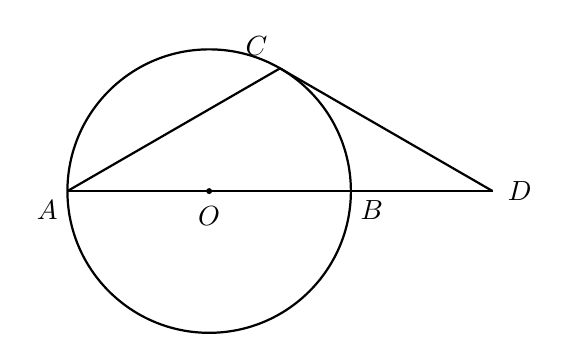
\begin{tikzpicture}[scale=0.9]
  % 半径 R=2，圆心 O=(2,0)；C 在圆心角 60° 处：C=(2+2cos60°, 2sin60°)=(3,1.732)
  % 切线 CD 与 x 轴交于 D=(6,0)
  \coordinate (A) at (0,0);
  \coordinate (O) at (2,0);
  \coordinate (B) at (4,0);
  \coordinate (C) at (3,1.732);
  \coordinate (D) at (6,0);
  \draw[thick] (O) circle (2);
  \draw[thick] (A) -- (D);
  \draw[thick] (A) -- (C);
  \draw[thick] (C) -- (D);
  \fill (O) circle (1.2pt) node[below=2pt] {$O$};
  \node[below left] at (A) {$A$};
  \node[below right] at (B) {$B$};
  \node[above left=1pt] at (C) {$C$};
  \node[right=2pt] at (D) {$D$};
\end{tikzpicture}
\end{center}
\nopagebreak[4]
\end{question}
\begin{question}
\gkti{9}\textbf{（12 分）} 证明：如果两数的和为一定值，那么当两数相等时，它们的乘积最大。

\end{question}